\begin{example}[קבצים]
רוצים למצוא (ולהדפיס) את כל קבצי התמונות ששמורות על הכונן הקשיח.
\end{example}
למשל עבור:
\begin{center}
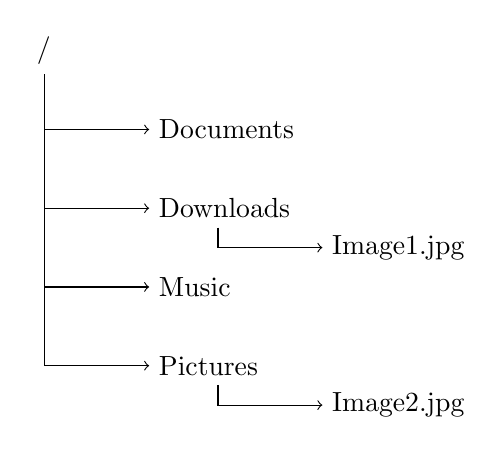
\begin{tikzpicture}[every node/.style={
	rectangle
%	, minimum width=1.5cm
%	, draw
	, text width=1.5cm
	, x=2.2cm
}, ->]

\node[text width=2mm](0) at(0,1) {/};
\foreach [count=\i] \x \y \name in {
	1/0/Documents
	, 1/-1/Downloads
	, 1/-2/Music
	, 1/-3/Pictures
	, 2/-1.5/Image1.jpg
	, 2/-3.5/Image2.jpg	
}{
	\node(\i) at(\x, \y) {\name};
}

\foreach \i in {1,...,4}{
	\draw (0) |- (\i);
}
\draw (2) |- (5);
\draw (4) |- (6);

\end{tikzpicture}
\end{center}

\begin{example}[מבוך]
נתון מבוך, נקודת התחלה ונקודת סוף ורוצים למצוא מסלול מנקודת ההתחלה לנקודת הסיום.
\end{example}

\begin{center}
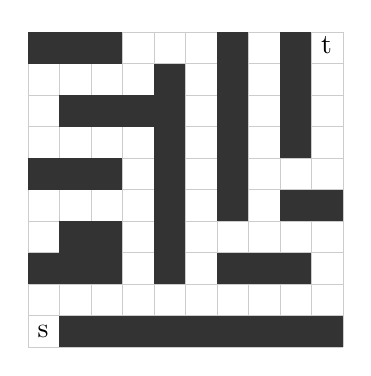
\begin{tikzpicture}

\def\dim{4mm}

\begin{scope}[x=\dim,y=\dim]
\draw[step=\dim,very thin, gray!40] (0,0) grid (10,10);

\foreach \a\b\c\d in{
	1/0/10/1
	,0/2/1/3
	,1/2/3/4
	,4/2/5/9
	,6/2/9/3
	,0/5/3/6
	,1/7/4/8
	,0/9/3/10
	,6/10/7/4
	,8/4/10/5
	,8/10/9/6
}{
	\fill[black!80] (\a,\b) rectangle (\c,\d);
}
\node[above right, rectangle] at(0,0) {s};
\node[above right, rectangle] at(9,9) {t};
\end{scope}

\end{tikzpicture}
\end{center}


\begin{example}[פאזל הזזה]
נתון לוח משחק בגודל 
$n \times m$
על הלוח 
$nm - 1$
חלקים ממוספרים מ-1 עד 
$nm - 1$
ומשבצת ריקה.
נתון סידור ראשוני של החלקים ואנו רוצים לסדר את החלקים לפי הסדר 
כך שבכל שלב מותר לנו להזיז את אחד החלקים ששכנים למשבצת הריקה אל המשבצת הריקה.
\end{example}
למשל עבור
$n = m = 3$:
\begin{center}
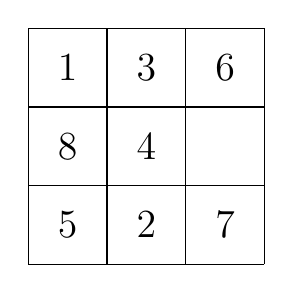
\begin{tikzpicture}
\draw (0,0) grid (3,3);

\begin{scope}[xshift=.5cm, yshift=.5cm, font=\Large]
\foreach \x \y \i in {0/0/5, 1/0/2, 2/0/7, 0/1/8, 1/1/4, 0/2/1, 1/2/3, 2/2/6}{
	\node at(\x, \y) {\i};
}
\end{scope}

\end{tikzpicture}
\end{center}

נראה בהמשך שאפשר לייצג כל אחת מהבעיות הנ"ל באמצעות גרף,
ומציאת הפתרון לכל אחת מהבעיות מבוסס על סריקה של הגרף המתאים.
כיצד עלינו לסרוק כל אחד מהגרפים המתאימים?

